\documentclass{protokol}
\leftheader{Určení měrného náboje elektronu}
\centerheader{Praktikum IV}
\rightheader{Tomáš Derner}

\begin{document}

  \section*{Úkol}

    \begin{enumerate}
      \item Změřte V-A charakteristiky magnetronu při konstantním magnetickém poli. Rozsah napětí na magnetronu volte $0 - \SI{200}{V}$ (s minimálním krokem $\num{0.1}-\SI{0.3}{V}$ v oblasti skoku). Proměřte $10 - 15$ charakteristik v rozsahu magnetizačních proudů $0 - \SI{2}{A}$.
      \item Pro každou naměřenou charakteristiku (při daném magnetickém poli) určete hodnotu kritického napětí (např. numerickou derivací). Získané hodnoty zpracujte graficky (pou\-žijte závislost kritického napětí na druhé mocnině magnetizačního proudu, absolutní člen získané lineární závislosti interpretujte jako kontaktní rozdíl potenciálů UK mezi materiály katody a anody) a ze směrnice určete měrný náboj elektronu. Diskutujte přesnost výsledku.
      \item Z naměřeného souboru dat vytvořte jeden graf závislosti anodového proudu magnetronem $I_A$ na magnetické indukci $B$ při konstantním anodovém napětí $U_A$ a popište jej. Rozmyslete si předem, jak musí být zvolené magnetizační proudy při měření anodových charakteristik, aby bylo možné určit sklon této charakteristiky v okolí kritické magnetické indukce $B_{kr}$.
    \end{enumerate}

  \section*{Teorie}

    V tomto praktiku pracujeme s magnetronem, který se skládá ze dvou soustředných válců tvořících elektrody usazených v magnetickém poli dvou cívek napájených proudem $I_{mag}$. Schéma a bližší popis lze nalézt v \cite{pokyny}.

    Měrným nábojem elektronu myslíme jeho elektrický náboj dělený hmotností.  Dle \cite{pokyny} lze měrný náboj vypočítat ze vztahu

    \begin{equation}
      \frac{e}{m_e} = \frac{ 8 U_{kr} }{ B_{kr}^2 r_A^2 } 
        \frac{ 1 }{ \left( 1 - \frac{ r_K^2 }{ r_A^2 } \right)^2 },
    \end{equation}
    kde $U_{kr}$ je kritické napětí, při kterém dopadají elektrony na anodu tečně, $B_{kr}$ kritická magnetická indukce, $r_A$ poloměr anody a $r_K$ poloměr katody. Při měření používáme konstantní magnetické pole dané vztahem
    \begin{equation}
      B = \frac{ 8 \mu_0 }{ 5 \sqrt{5} } \frac{ N I_{mag} }{ \rho_0 },
    \end{equation}
    kde $\mu_0 = \SI{4 \pi e-7}{\henry\per\metre}$ je permeabilita vakua, $N$ počet závitů každé cívky a $\rho_0$ jejich střední poloměr.

    Podle těchto vztahů se dá tedy měrný náboj určit lineární regresí vztahu 
    \begin{equation} \label{eq:fit}
      U_{kr} = a I_{mag}^2 + U_k,
    \end{equation}
    kde $U_k$ je konstantní kontaktní rozdíl potenciálů mezi materiály katody a anody a $a$ je dáno vztahem 
    \begin{equation} \label{eq:a}
      a = \frac{ e }{ m_e } \frac{ 8 \mu_0^2 N^2 r_A^2 }{ 125 \rho_0^2 }
        \left( 1 - \frac{ r_K^2 }{ r_A^2 } \right)^2.
    \end{equation}
    
    \begin{figure}[H]
      \centering
      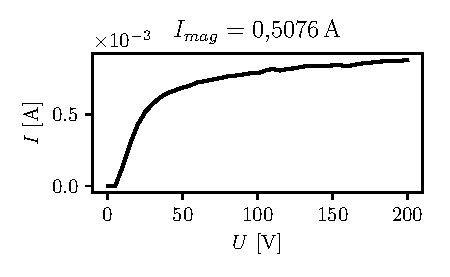
\includegraphics[]{u1_05A_5Vs}
      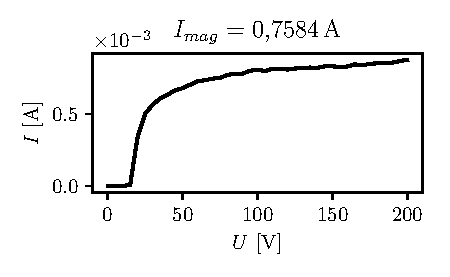
\includegraphics[]{u1_075A_5Vs}\\ \vspace{-15px}
      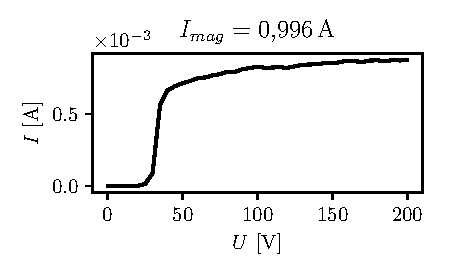
\includegraphics[]{u1_1A_5Vs}
      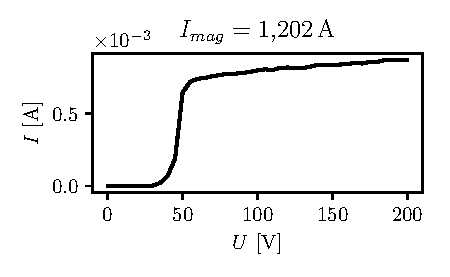
\includegraphics[]{u1_12A_5Vs}\\ \vspace{-15px}
      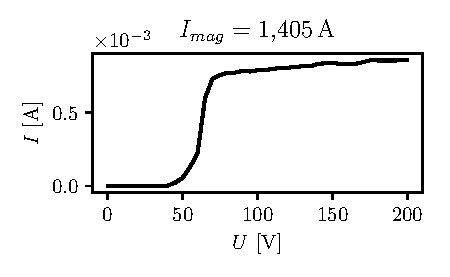
\includegraphics[]{u1_14A_5Vs}
      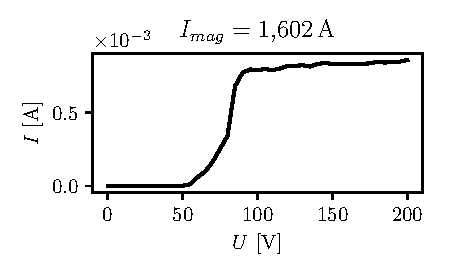
\includegraphics[]{u1_16A_5Vs}\\ \vspace{-15px}
      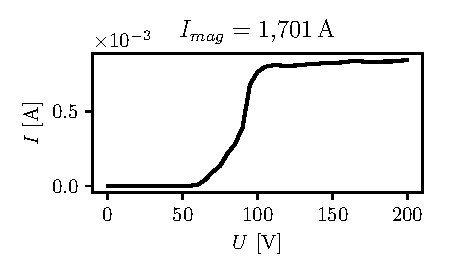
\includegraphics[]{u1_17A_5Vs}
      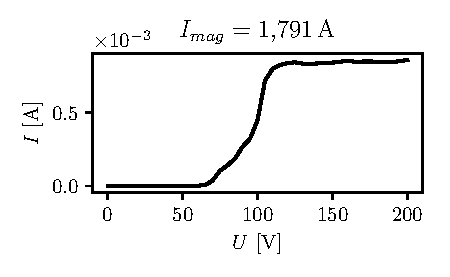
\includegraphics[]{u1_18A_5Vs}\\ \vspace{-15px}
      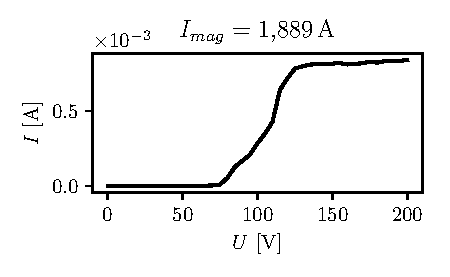
\includegraphics[]{u1_19A_5Vs}
      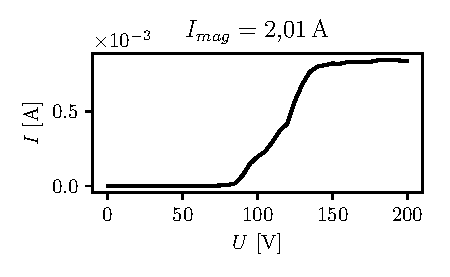
\includegraphics[]{u1_2A_5Vs} \vspace{-15px}
      \caption{Grafy voltampérových charakteristik pro úkol 1}
      \label{fig:u1}
    \end{figure} 

  \section*{Výsledky} 

    Použitá sestava měla parametry $r_A = \SI{5.00 \pm 0.05}{mm}$, $r_K = \SI{0.19 \pm 0.01}{mm}$, $N = 630$ a $\rho_0 = \SI{75}{mm}$.

    \subsection*{Úkol 1}

      Bylo naměřeno 10 voltampérových charakteristik s napětím v rozsahu $0 -   \SI{200}{V}$ s krokem $\SI{5}{V}$ a s magnetizačním proudem v intervalu $ \num{0.5} - \SI{2}{A} $. Výsledné charakteristiky jsou  vyneseny v grafech na obrázku \ref{fig:u1}. 

    \subsection*{Úkol 2} 

      Pomocí numerické derivace v programu Origin v praktiku byla určena kritická napětí pro závislosti naměřené v úkolu 1. Pro jejich přesnější určení byla okolí inflexního bodu proměřena podrobněji s krokem $\SI{0.2}{V}$. Za hodnoty kritických napětí byly vzaty maxima grafů derivací, chyby byly určeny jako polovina šířky píku v jeho polovině, přičemž polovina píku byla určena odhadem. Výsledky jsou shrnuty v tabulce

      \begin{table}[H]
        \centering
        \setlength{\tabcolsep}{10pt}
        \begin{tabular}[t]{
  S[table-format=1.3]
  S[table-format=3.1]
  S[table-format=1.1]
} \toprule
{$I_{mag}$} & {$U_{kr}$} & {$\sigma_{U_{kr}}$} \\
{[A]}       & {[V]}      & {[V]}               \\ \midrule
      0.508 &        8.4 &                 0.5 \\
      0.758 &       19.4 &                 0.8 \\
      0.996 &       32.8 &                 1.0 \\
      1.202 &       47.0 &                 0.7 \\
      1.405 &       64.0 &                 0.7 \\
      1.602 &       82.6 &                 0.7 \\
      1.701 &       92.4 &                 0.8 \\
      1.791 &      101.8 &                 0.7 \\
      1.889 &      112.0 &                 1.0 \\
      2.010 &      124.3 &                 1.1 \\ \bottomrule
\end{tabular}
        \caption{Tabulka kritických napětí pro různé magnetizační proudy}
        \label{tab:u2}
      \end{table}

      V grafu na obrázku \ref{fig:u2} je zobrazena závislost kritického napětí na druhé mocnině magnetizačního proudu, proložená lineárním fitem \eqref{eq:fit}. Níže jsou uvedeny fitové konstanty. K chybě fitu obou konstant byla přičtena chyba určení kritického napětí aproximovaná hodnotou $\SI{1}{V}$.
      
      $$ a = \SI{30.9 \pm 1.3}{\volt\per\ampere\squared}, $$
      $$ U_k = \SI{2.0 \pm 1.8}{\volt}. $$

      Pomocí vztahu \eqref{eq:a} a hodnot konstant uvedených v úvodu sekce výsledků byl určen měrný náboj elektronu 
      $$ \frac{ e }{ m_e } = \SI{1.74 \pm 0.08 e+11}{\coulomb\per\kilogram}. $$ 
      Tato hodnota se shoduje v rámci chyby s hodnotou uvedenou v \cite{pokyny}.

      \begin{figure}[H]
        \centering
        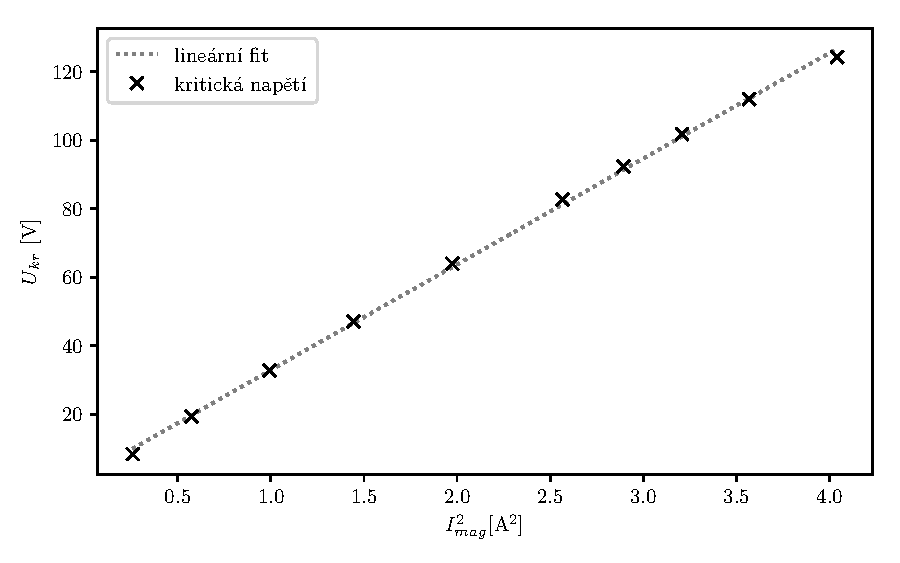
\includegraphics[]{u2}
        \caption{Závislost $U_{kr} = U_{kr}(I_{mag}^2)$}
        \label{fig:u2}
      \end{figure}

    \subsection*{Úkol 3}

      Graf \ref{fig:u3} zobrazuje hodnoty zásislosti proudu magnetronem na magnetické indukci při konstantním napětí.

      \begin{figure}[H]
        \centering
        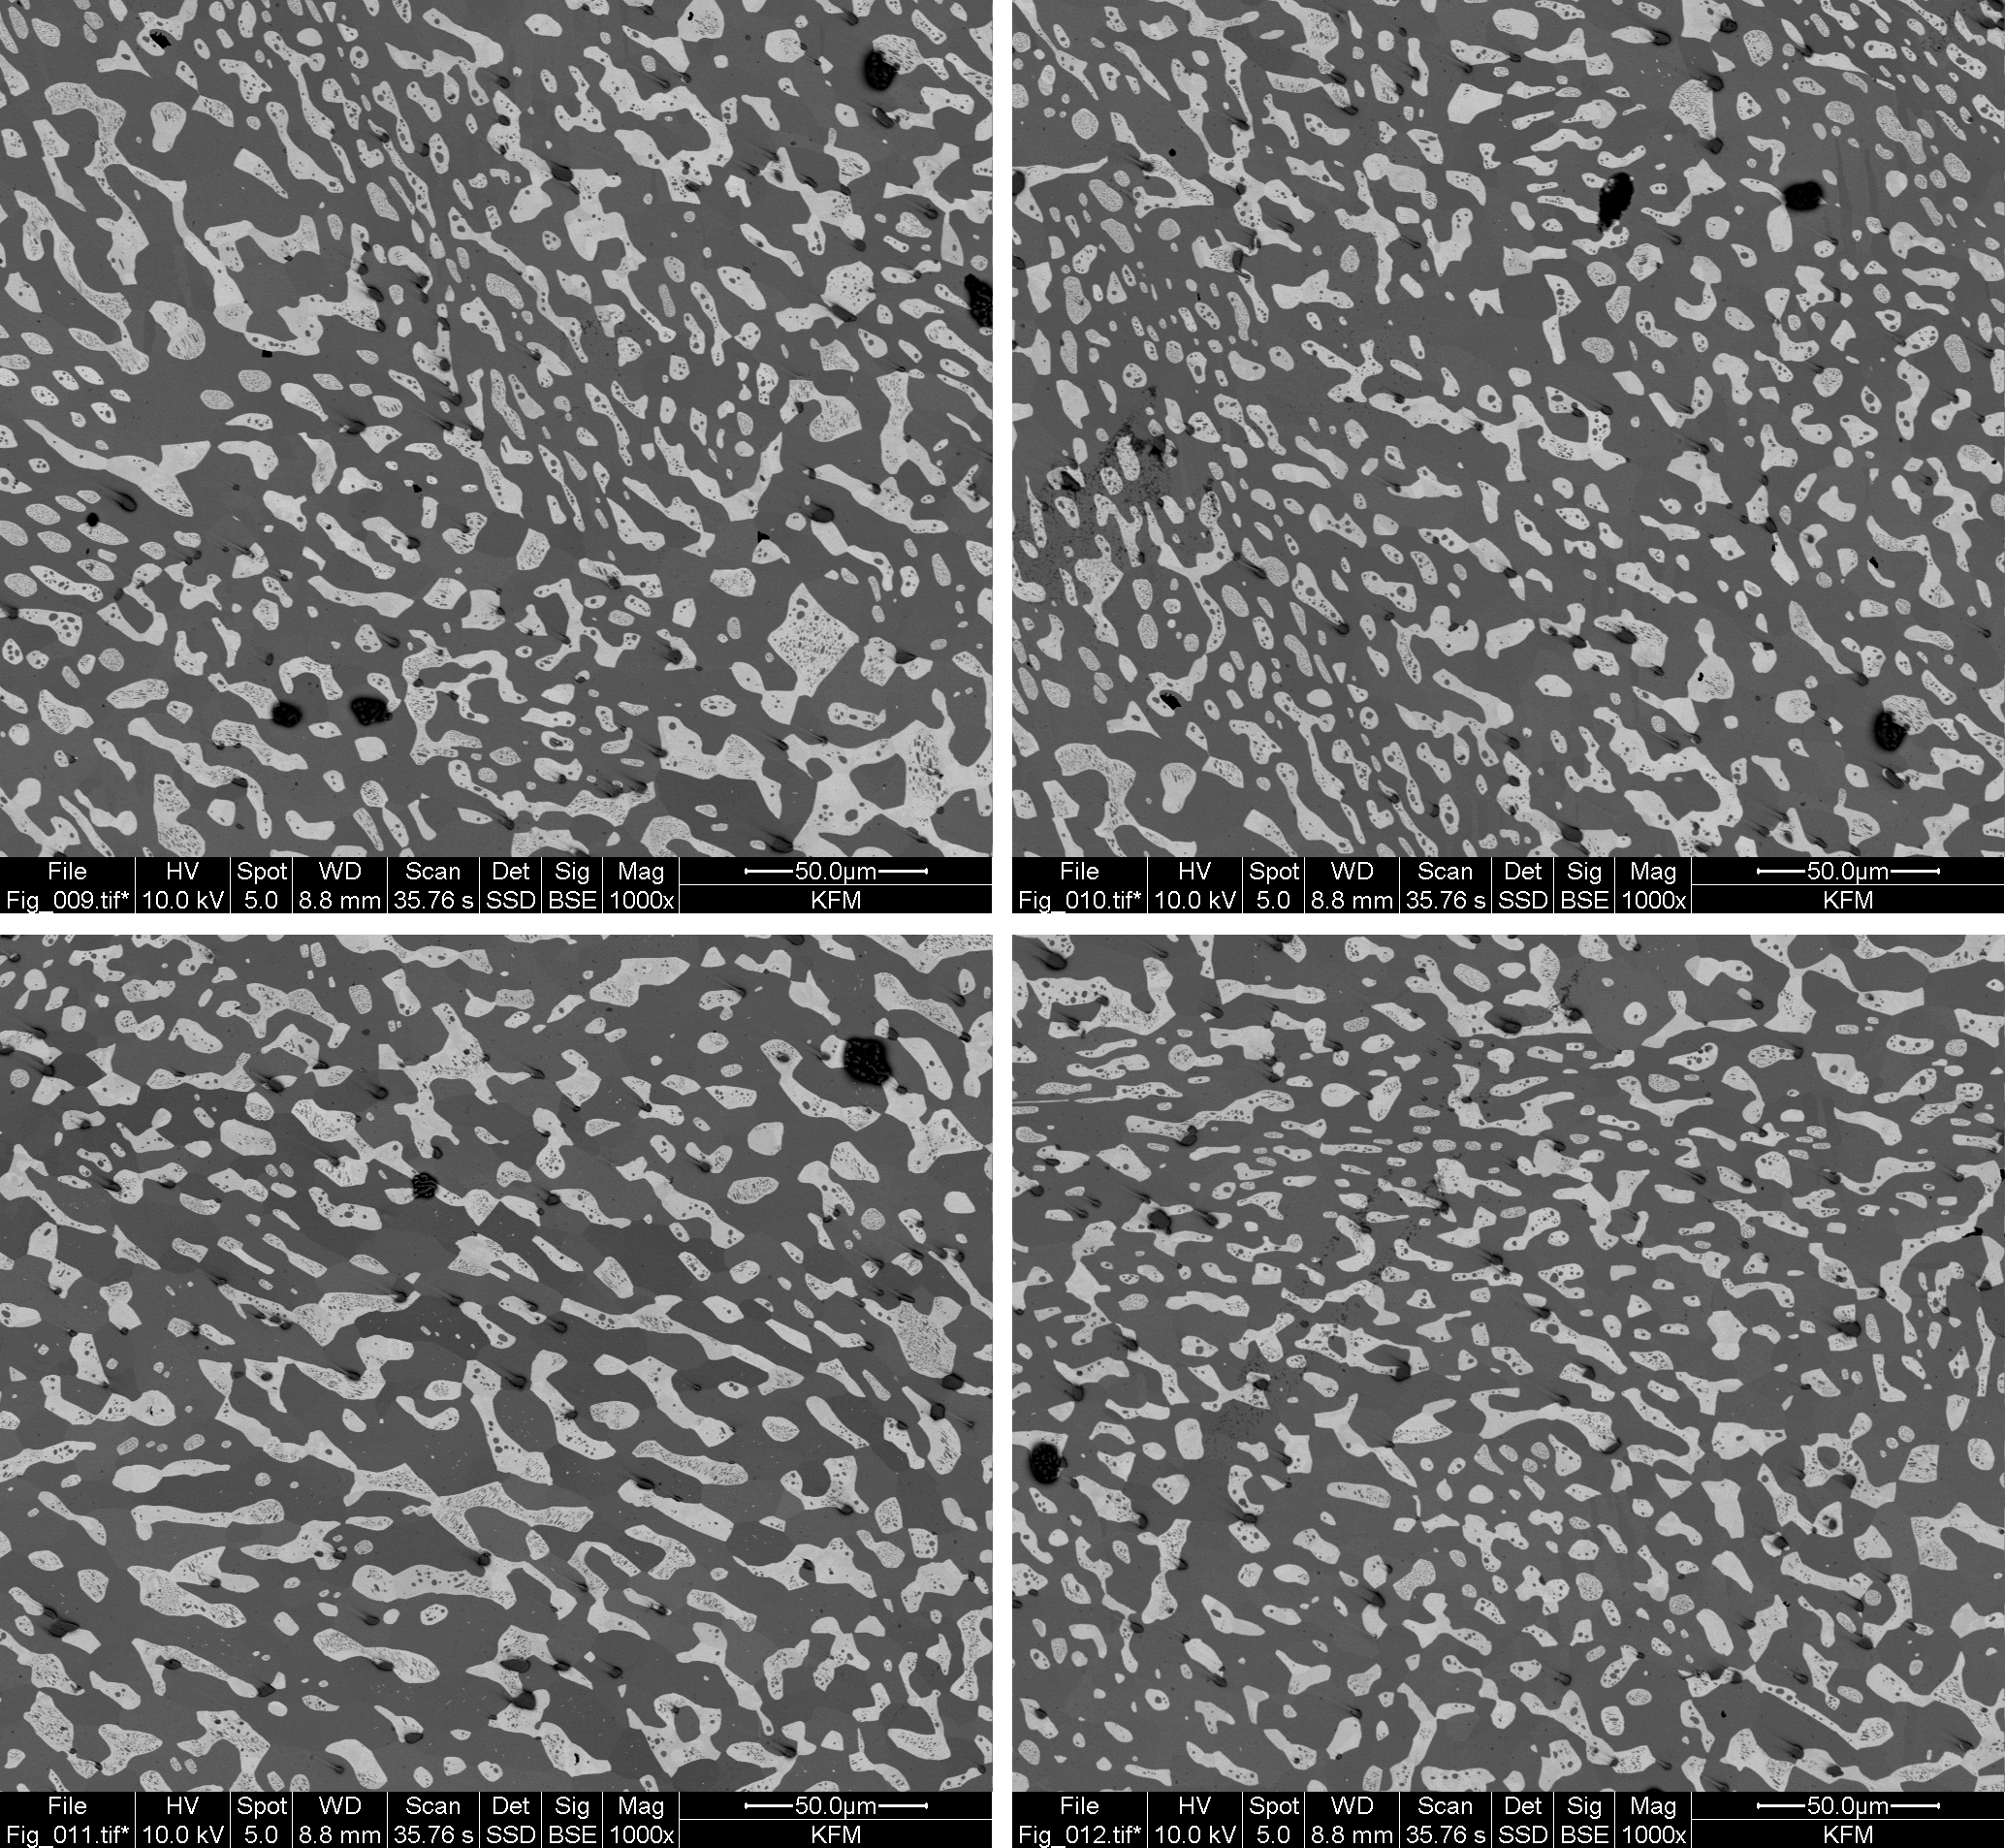
\includegraphics[]{u3}
        \caption{Závislost proudu magnetronem na magnetické indukci při $U = \SI{30}{V}$}
        \label{fig:u3}
      \end{figure}

  \section*{Diskuse}

    Výsledná hodnota měrného náboje se v rámci chyby shoduje s hodnotou uvedenou v \cite{pokyny}. Uvedená chyba je však poměrně vysoká. To je způsobeno především  nepřesným určením kritických napětí pomocí numerické derivace, respektive způsobem určování chyby těchto hodnot. 

    V chybě výsledku se skryly faktory ztěžující přesné měření měrného náboje, například skutečnost, že magnetická indukce zde byla vyjádřena aproximativním vzorcem, či vliv nedokonalosti vakua v magnetronu.

  \section*{Závěr}

    Naměřené charakteristiky odpovídají teoretickým předpovědím. Pomocí nich byla určena hodnota měrného náboje elektronu 
    $$ \frac{ e }{ m_e } = \SI{1.74 \pm 0.08 e+11}{\coulomb\per\kilogram}. $$
    Tato hodnota odpovídá v rámci chyby hodnotě tabulkové.

  \begin{thebibliography}{}
 
    \bibitem{pokyny}
    Pokyny k měření ``Určení měrného náboje elektronu z charakteristik magnetronu'', dostupné z\\ \url{https://physics.mff.cuni.cz/vyuka/zfp/_media/zadani/texty/txt_413.pdf}, 16.\,10.\,2018
   
  \end{thebibliography}

\end{document} 